\documentclass[a4paper]{article}
\usepackage{mathtools}
\usepackage{listings}
\usepackage{graphicx}
\usepackage{float}
\usepackage{amsmath}
\usepackage[font=it, width=0.9\linewidth]{caption}
\usepackage{bm}
\usepackage[hidelinks]{hyperref}
% \usepackage{placeins} %non fa andare le figure in una sezione nella sezione dopo%
% \usepackage[italian]{babel}
\newcounter{count_es}
\newcounter{count_sub_es}[count_es]
% \captionsetup[figure]{name=Fig.}
\renewcommand{\figurename}{Fig.}
\renewcommand{\tablename}{Tab.}

\begin{document}
\title{Relazione di laboratorio: algebra lineare}
\author{Samuele Bellini}
\date{17 Settembre 2025}
\maketitle

\stepcounter{count_es}
\section*{Esercizio \arabic{count_es} - Algebra delle matrici}

\stepcounter{count_sub_es}
\subsection*{ (\alph{count_sub_es})}
Data la matrice:
\[A = \begin{bmatrix}
        -1 & 1 \\
        -1 & -1 
    \end{bmatrix}\]
è possibile ricavarne gli autovalori e i corrispondenti 
autovettori utilizzando la funzione presente nel  pacchetto 
NumPy di Python: \lstinline{np.linalg.eig(A)}. \\
Si ottengono così gli autovalori:
\begin{subequations}    
    \begin{align*}
        \lambda_{1} = (-1+i)\\
        \lambda_{2} = (-1-i)
    \end{align*}
\end{subequations}
e i corrispondenti autovettori:
\begin{subequations}    
    \begin{align*}
        \mathbf{v_{1}} &= (0.70710678, 0.70710678i)\\
        \mathbf{v_{2}} &= (0.70710678, -0.70710678i).
    \end{align*}
\end{subequations}

Si può poi calcolare la matrice esponenziale \(e^{At}\),
in funzione del parametro reale \(t\), tramite la relazione:
\[e^{At} = Ue^{Dt}U^{-1},\] 
dove \(U\) è la matrice degli autovettori di \(A\), \(D\) è
la diagonalizzazione di A ed 
\(e^{Dt} = \bigl[\begin{smallmatrix} e^{\lambda_{1}t}&0 \\ 0&e^{\lambda_{2}t} \end{smallmatrix}\bigr]\).
Si riportano i valori degli elementi della matrice esponenziale 
\(e^{At}\) in funzione di \(t\in[0,5]\) in \figurename~\ref{fig:es_1a}. Si può così osservare
che i valori della matrice sono sempre reali e che, per \(t=0\), \(e^{At} = I_{2}\). 
\\Questi risultati risultano verificati anche analiticamente, in quanto si 
può ricavare che:
\[e^{At} = e^{-t}\bigl[\begin{smallmatrix}
    \cos(t)&\sin(t)\\-\sin(t)&\cos(t)
\end{smallmatrix}\bigr].\]
\begin{figure}[H]
    \centering
    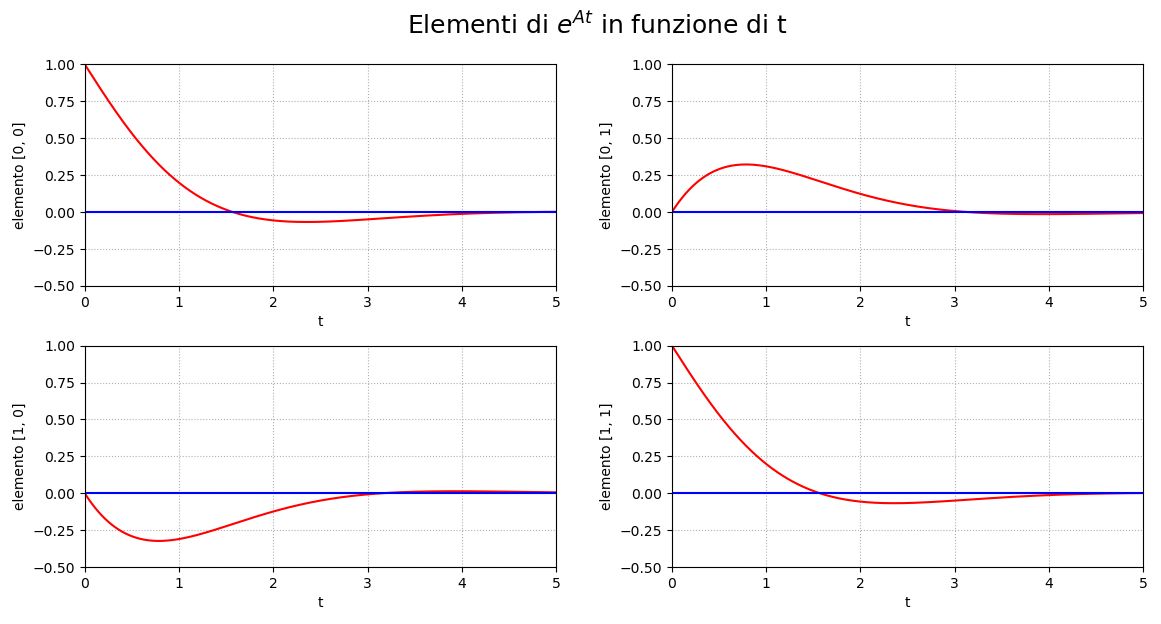
\includegraphics[width=.95\linewidth]{Es_1a.png}
    \caption{Grafici dei valori degli elementi di \(e^{At}\) in funzione di 
    \(t\) nell'intervallo [0,5]. In rosso è riportata la parte reale dell'elemento
    e in blu la parte immaginaria. \label{fig:es_1a}}
\end{figure}
\stepcounter{count_sub_es}
\subsection*{ (\alph{count_sub_es})}
Dopo aver generato delle matrici \(n \times n\) con gli elementi
presi da una distribuzione normale standard, operazione realizzabile
in Python tramite la linea di codice \lstinline{np.random.standard_normal((n,n))}, 
è possibile calcolarne gli autovalori e graficare questi ultimi (divisi per un fattore \(\sqrt{n}\))
nel piano complesso per osservare come per n piccoli i punti sono concentrati
principalmente sull'asse reale, mentre, al crescere di n, la distribuzione 
tende sempre più ad una distribuzione uniforme
all'interno del cerchio di raggio unitario. 
Si può osservare questo comportamento in \figurename~\ref{fig:es_1b}, dove sono
rappresentati 20\,000 autovalori per grafico, con dimensionalità n delle matrici quadrate crescente.\\
Per quantificare questo fenomeno si può calcolare il valore della varianza rispetto allo zero sia 
per la parte reale che per la parte immaginaria degli autovalori divisi per \(\sqrt{n}\); come ci si aspetta,
per n piccoli si ottengono valori piccoli della varianza della parte immaginaria e grandi per la parte
reale, mentre per n grandi le due varianze tendono sempre più a \(\frac{1}{4}\), che è la varianza attesa
per una distribuzione uniforme su un cerchio di raggio unitario. I valori di queste varianze sono riportati in
\tablename~\ref{tab:es_1b}.
\begin{table}[H]
    \centering
    \setlength{\tabcolsep}{10pt}  %column separation%
    \renewcommand{\arraystretch}{1.25} %row separation%
    \begin{tabular}{c | c | c}
        \textbf{n} & \(\bm{\sigma^{2}_{\mathrm{Re}}}\) & \(\bm{\mathbf{\sigma}^{2}_{\mathrm{Im}}}\) \\
        \hline
        4 & 0.415262 & 0.168300 \\
        10 & 0.309844 & 0.213243\\
        100 & 0.255770 & 0.245610\\
        1\,000 & 0.250076 & 0.249655\\
    \end{tabular}
    \caption{Valori delle varianze rispetto allo zero delle parti reali e immaginarie degli autovalori divisi per 
    \(\sqrt{n}\) con i rispettivi valori della dimensionalità n.
    \label{tab:es_1b}}
\end{table}
\begin{figure}[H]
    \centering
    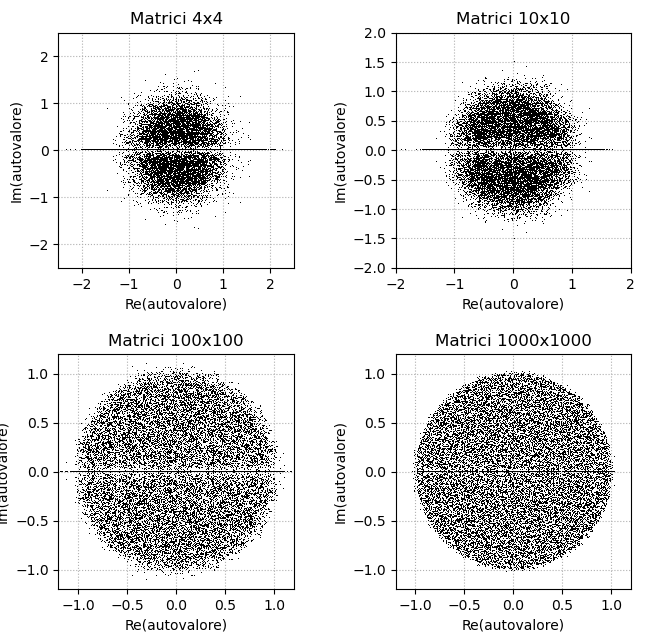
\includegraphics[width=.7\linewidth]{Es_1b.png}
    \caption{Grafici degli autovalori di matrici \(n \times n\), divisi per \(\sqrt{n}\),
    nel piano complesso; in ogni figura sono rappresentati 20\,000 autovalori, con n che assume i valori 4, 10, 100, 1\,000.  \label{fig:es_1b}}
\end{figure}
Si può verificare che, al posto di dividere gli autovalori per \(\sqrt{n}\), sarebbe stato equivalente generare
le matrici con elementi presi da una distribuzione normale con deviazione standard pari a \(\sqrt{n}\) e media nulla.
\stepcounter{count_sub_es}
\subsection*{ (\alph{count_sub_es})}
Dato un dataset di molecole è possibile calcolare i momenti d'inerzia
principali delle singole calcolando gli autovalori delle matrici momento d'inerzia:
\[ I = \begin{bmatrix}
            \displaystyle\sum_{i}^{} m_{i}(y_{i}^{2} + z_{i}^{2}) & -\displaystyle\sum_{i}^{} m_{i} x_{i} y_{i}  & -\displaystyle\sum_{i}^{} m_{i} x_{i} z_{i}\\
            -\displaystyle\sum_{i}^{} m_{i} x_{i} y_{i} & \displaystyle\sum_{i}^{} m_{i}(x_{i}^{2} + z_{i}^{2}) & -\displaystyle\sum_{i}^{} m_{i} y_{i} z_{i}\\
            -\displaystyle\sum_{i}^{} m_{i} x_{i} z_{i} & -\displaystyle\sum_{i}^{} m_{i} y_{i} z_{i} & \displaystyle\sum_{i}^{} m_{i}(x_{i}^{2} + y_{i}^{2})
        \end{bmatrix}, \]
dove \(m_{i}\) e \((x_{i}, y_{i}, z_{i})\) sono massa e posizione, relativa al centro di massa 
della molecola, dell'atomo i-esimo che compone la molecola. Per fare ciò, una volta che sono state
ricavate le posizioni degli atomi che compongono la molecola rispetto al centro di massa di quest'ultima e poi calcolata la matrice \(I\) della singola molecola,
basterà utilizzare la linea di codice \lstinline{np.linalg.eigvalsh(I)} per ricavare i momenti d'inerzia
principali, ordinati in ordine crescente. \\
Si possono poi classificare le molecole in base alle relazioni tra i momenti d'inerzia \(I_{a}, I_{b}, I_{c}\) (con \(I_{a} \leq I_{b} \leq I_{c}\)) secondo 
il seguente criterio:
\begin{description}
    \item [Sferica:] \(I_{a} = I_{b} = I_{c}\) 
    \item [Oblata:] \(I_{a} = I_{b} < I_{c}\) 
    \item [Prolata:] \(I_{a} < I_{b} = I_{c}\) 
    \item [Asimmetrica:] \(I_{a} < I_{b} < I_{c}\) 
\end{description}
Per fare ciò in Python si è preferito, invece di verificare che sussista l'uguaglianza esatta fra valori decimali, 
che darebbe risultati incorretti a causa delle imprecisioni dei floating~point, oltre a possibili imprecisioni nel dataset stesso,
andare a verificare che i valori dei momenti d'inerzia principali siano molto simili tramite la funzione \lstinline{math.isclose()}, nella quale
è stato passato 0.01 come valore di tolleranza relativa (si chiede quindi che la distanza fra i due valori sia minore o uguale all'1\% del valore massimo). \\
In questo modo è stato ottenuto il conteggio per categoria dal dataset fornito riportato in \tablename~\ref{tab:es_1c}.
\begin{table}[H]
    \centering
    \setlength{\tabcolsep}{10pt}  %column separation%
    \renewcommand{\arraystretch}{1.25} %row separation%
    \begin{tabular}{ c | c | c | c}
        \textbf{Sferica} & \textbf{Oblata} & \textbf{Prolata} & \textbf{Asimmetrica}\\
        \hline
         2 & 18 & 92 & 7053  \\
    \end{tabular}
    \caption{Numero di molecole per categoria dal dataset fornito.\label{tab:es_1c}}
\end{table}

\stepcounter{count_es}
\section*{Esercizio \arabic{count_es} - Decomposizione SVD}
\stepcounter{count_sub_es}
\subsection*{ (\alph{count_sub_es})}
Data la matrice:
\[A = \begin{bmatrix}
        0 & 1 & 0 & 0 \\
        0 & 0 & 2 & 0 \\
        0 & 0 & 0 & 3 \\
        \epsilon & 0 & 0 & 0 \\
    \end{bmatrix}\]
è possibile valutare come i suoi autovalori e valori singolari varino per piccole
perturbazioni del parametro \(\epsilon\). Come caso di studio è stato preso \(\epsilon \in [0, 10^{-5}]\).
Per calcolare i valori singolari di \(A\) è stata utilizzata la funzione
\lstinline{np.linalg.svd(A)[1]}, dove con [1] si seleziona il secondo oggetto 
restituito dalla funzione \lstinline{svd}, che corrisponde al vettore di valori singolari.
Per calcolare gli autovalori di \(A\), invece, è stata utilizzata la funzione
\lstinline{np.linalg.eigvals(A)}, la quale restituisce direttamente il vettore di autovalori.
I risultati di queste operazioni sono riportati in \figurename~\ref{fig:es_2a}.
Si osserva così che i primi tre valori singolari rimangono costanti su tutto
l'intervallo, mentre il quarto è sempre pari al valore della perturbazione \(\epsilon\); 
gli autovalori, invece, sono sempre reali o immaginari puri, e la relazione fra \(\epsilon\) e 
la parte non nulla è la stessa per ogni autovalore, a meno di riflessioni rispetto all'asse reale.
\begin{figure}[H]
    \centering
    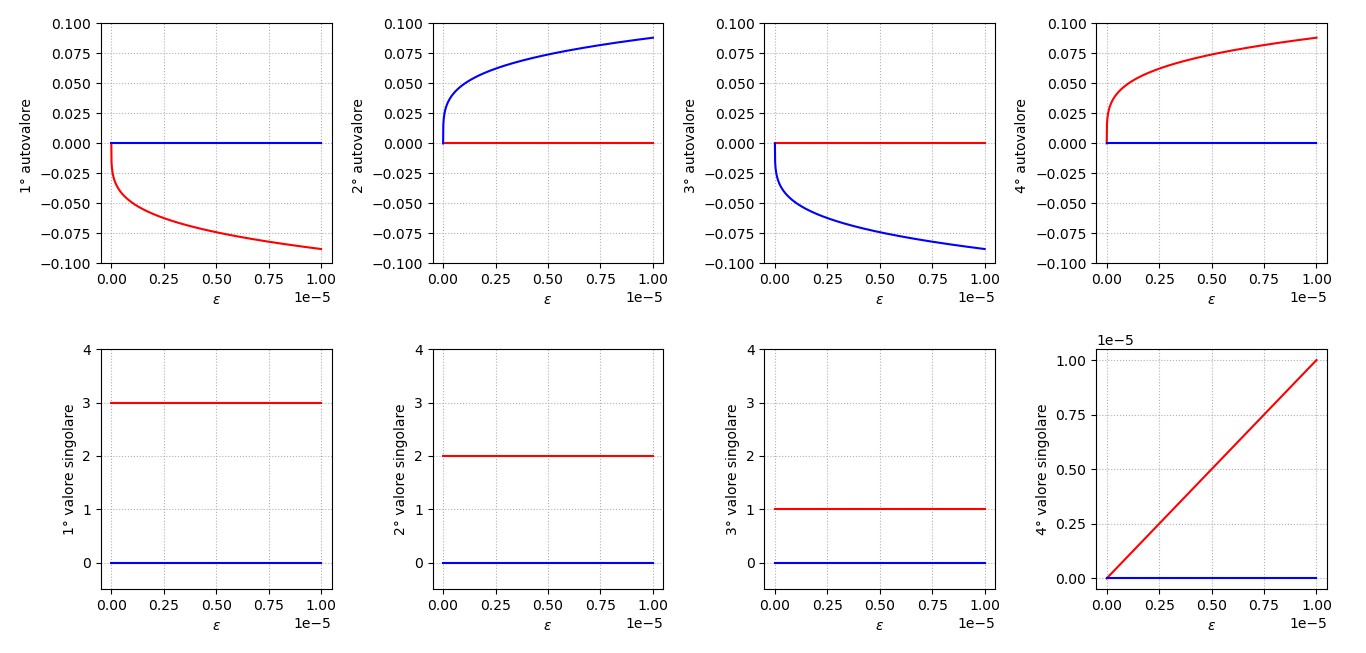
\includegraphics[width=.95\linewidth]{Es_2a.png}
    \caption{Grafici degli autovalori e dei valori singolari di \(A\) in funzione della 
    perturbazione \(\epsilon\); i primi sono riportati nella prima riga, i secondi nella successiva.
    In rosso sono riportate le parti reali, in blu le parti immaginarie. Si faccia attenzione 
    al cambio di scala per il quarto valore singolare rispetto ai primi tre.\label{fig:es_2a}}
\end{figure}    
\stepcounter{count_sub_es}
\subsection*{ (\alph{count_sub_es})}
Data un'immagine è possibile rappresentarla come un insieme di tre matrici reali
con elementi \(\in [0,1]\), rappresentanti le componenti rosso, verde e blu dei pixel che
compongono l'immagine. Per studiare l'andamento dei valori singolari delle matrici e come appare
l'immagine a vari livelli di accuratezza si potrebbe andare a lavorare sulla versione in bianco e nero dell'immagine,
in modo da avere un'unica matrice, ma così facendo si perderebbero le informazioni cromatiche; per mantenere queste informazioni e ricavarne
infine un'immagine a colori si è preferito studiare singolarmente le tre componenti, per poi ricavarne l'immagine complessiva ricombinandole.
Innanzitutto è stata calcolata l'SVD per ogni matrice delle componenti che compone l'immagine scelta (riportata in \figurename~\ref{fig:es_2b_1} a sinistra) tramite
la linea di codice \lstinline{np.linalg.svd(img_i, full_matrices=True)},
dove img\_i rappresenta una delle tre matrici di componenti, ed è stata graficata la somma cumulativa normalizzata dei valori singolari delle singole matrici in \figurename~\ref{fig:es_2b_1} a destra. 
Si osserva così che l'andamento dei valori singolari è pressocché identico per tutte le componenti, come ci si aspetta
da un'immagine in cui non sono presenti preferenze per nessuna componente specifica (in un'immagine completamente rossa, ad esempio, si trovano 
valori singolari nulli per le componenti blu e verdi e non nulli solo nella componente rossa), e che la stragrande maggioranza dell'informazione è
contenuta in pochi valori singolari; questo è evidente in \figurename~\ref{fig:es_2b_1} a destra, dove si può osservare come, con appena un terzo dei
valori singolari (circa 250 su 700), la somma cumulativa ha già superato il 90\% del suo valore massimo.
\begin{figure}[H]
    \centering
    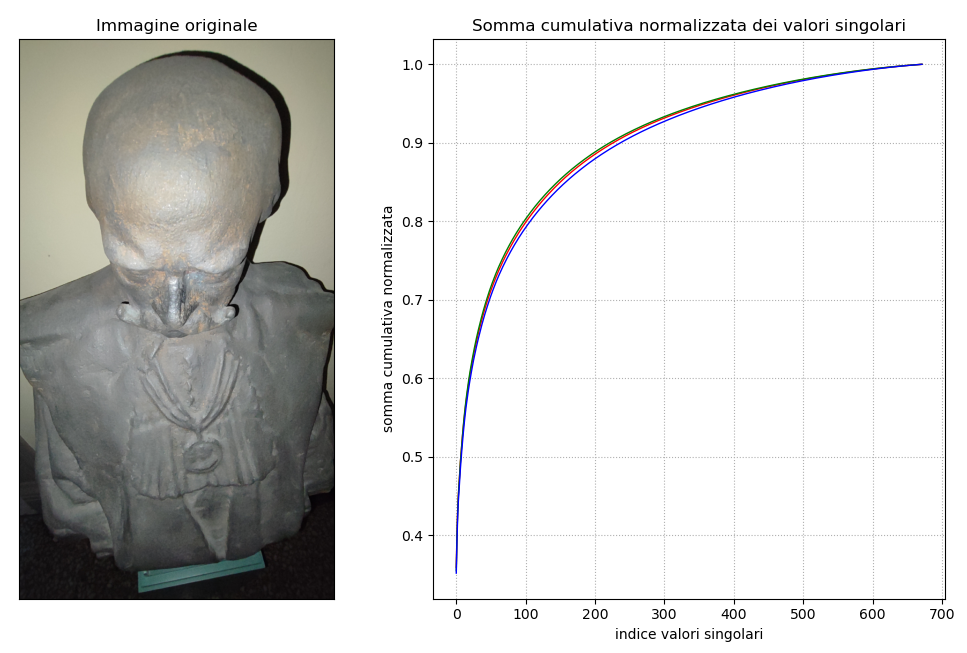
\includegraphics[width=.75\linewidth]{Es_2b_1.png}
    \caption{A sinistra l'immagine originale, a destra il grafico delle somme cumulative normalizzate
    dei valori singolari delle singole componenti cromatiche, dove il colore della linea indica la rispettiva componente.\label{fig:es_2b_1}}
\end{figure}
Sapendo come variano i valori singolari si può scegliere un valore di cutoff, \(r \in {1, 2, ..., 700}\) 
(il massimo valore di r è 700 perché, per questa immagine, è il valore minimo tra larghezza e altezza, in pixel, dell'immagine), che indica il numero di 
valori singolari che verranno utilizzati per ricostruire l'immagine dalla decomposizione SVD delle componenti. 
Si riporta, in \figurename~\ref{fig:es_2b_2}, il risultato di questa operazione per \(r=3,20,100,500\), 
assieme alla differenza fra l'immagine originale e la ricostruzione. Dalle figure si osserva bene come per valori di \(r\) molto piccoli la ricostruzione
è molto grossolana e mantiene solo le forme essenziali, per valori di \(r\) più grandi si perdono solo piccoli dettagli, e come, per \(r=500\),
nella differenza rimane quasi esclusivamente rumore. Si noti anche che, nonostante l'utilizzo di molti più dati per ricostruire l'ultima immagine, la 
differenza fra questa e la penultima sia minimale, evidenziando quindi come sia superfluo andare a utilizzare un numero così elevato di valori 
singolari, in quanto quasi tutta l'informazione è racchiusa in quelli precedenti.
\begin{figure}[H]
    \centering
    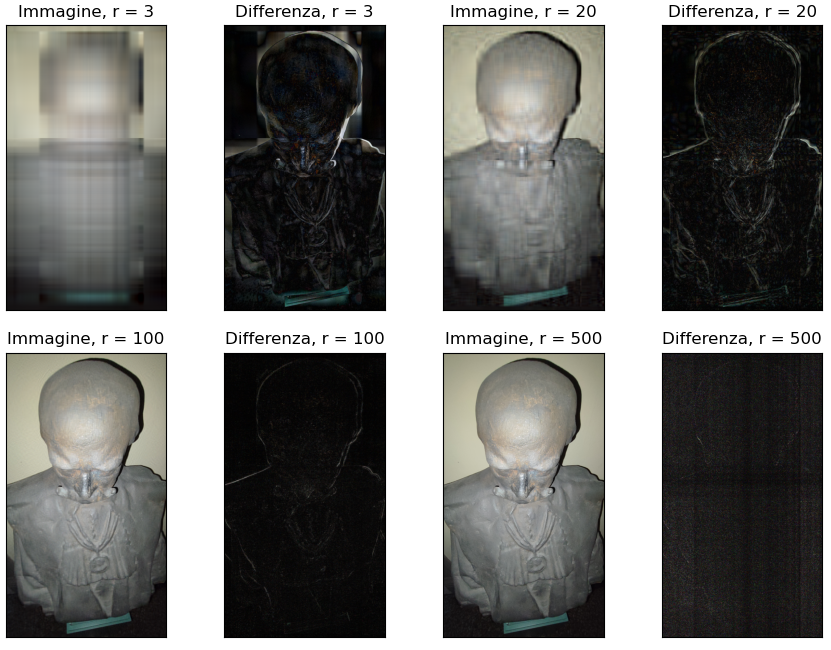
\includegraphics[width=.95\linewidth]{Es_2b_2.png}
    \caption{Ricostruzione dell'immagine per r = 3, 20, 100, 500 con la rispettiva differenza (in valore assoluto) dall'immagine originale. Si noti che
    nelle immagini della differenza è stato massimizzato il contrasto per renderle più visibili. \label{fig:es_2b_2}}
\end{figure}
\section*{Codice}
Il codice utilizzato per risolvere gli esercizi è consultabile su GitHub al link: \url{https://github.com/saemmie4/Lab-Data-Science}

\end{document}